\chapter{Allgemeine Einführung}
In diesem Kapitel wird auf die zugrunde liegende Theorie bezüglich Bildverarbeitung, Marching Cubes, verwendete Dateiformate und OpgenGL eingegangen. Es wird ein grober Überblick über die wichtigsten Begrifflichkeiten der jeweiligen Bereiche geschaffen, um ein grundlegendes Verständnis der Materie zu gewährleisten. Da es sich jeweils um sehr große Bereiche handelt wurde darauf geachtet nur das wesentliche welches für das Verständnis dieser Arbeit notwendig ist zu erfassen.
\section{Bildgebende Verfahren}
\begin{quote}
	''Die Medizinische Bildverarbeitung hat das Ziel, medizinische Bilder und Bildfolgen zur Unterstützung der medizinischen Diagnostik und Therapie aufzubereiten, zu analysieren und zu visualisieren.'' \citep{MedBildVerarbeitung}\\
\end{quote}
Die verschiedenen medizinischen Verfahren können grob in die Art der erzeugten Bilddaten eingeteilt werden.\\
\begin{itemize}
	\item \textbf{Schnittbilder} z.B. mittels Computertomografie, Magnetresonanztomografie oder Röntgentomografie.
	\item \textbf{Projektionsbilder} z.B. durch ''klassisches'' Röntgen.
	\item \textbf{Oberflächenabbildungen} z.B. durch Rastertunnelmikroskop.\\
\end{itemize}
Das Hauptaugenmerk dieser Arbeit liegt auf der aus den tomographischen Verfahren erhaltenden Schnittbildern, welche als sogenannte Voxel-Modelle gespeichert werden. Ein vollständiges dreidimensionales Bild besteht aus mehreren solcher übereinandergelegten Schnittbildern.

\section{Volumengrafik}
Unter Volumengrafik versteht man in der Computergrafik die Darstellung von Objekten durch eine Menge von Punkten. Diese Punkte werden auch als Voxeln bezeichnet und repräsentieren einen Punkt im Raum.
\subsection{Voxel} 
Ein solches Voxel ist als ein einzelner Punkt in einem dreidimensionalen Objekt zu verstehen, welcher einen gewissen Isowert aufweist. Dieser Wert beschreibt die Eigenschaft des Objektes an diesem Punkt und ist essentiell um z.B. bei den tomographischen Verfahren in der Medizin die festeren von den weicheren teilen eines Körpers zu unterscheiden (z.B. Knochen und Gewebe). In Abbildung \ref{fig:Voxelgitter} ist eine solche Voxel-Menge zusehen die verschiedenen Grauwerte der einzelnen Bildpunkte stellen dabei die unterschiedlichen Isowerte dar.

\begin{figure}
	\centering
	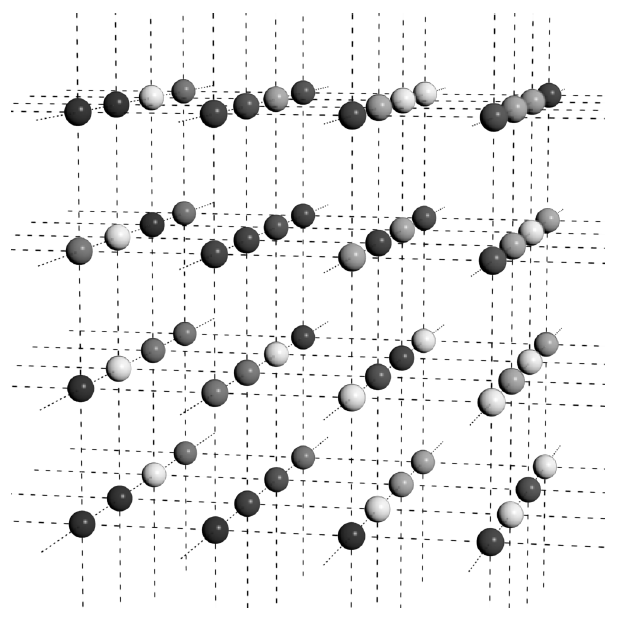
\includegraphics[width=.85\textwidth]{Voxelgitter}
	\caption{Ein Voxelgitter \citep{SeibtBak}.}
	\label{fig:Voxelgitter}
\end{figure}

\section{Marching Cubes}
Da der Marching Cubes Algorithmus das zentrale Element dieser Arbeit bildet, wird hier seine Grundform wie sie in \citep{MCAlgo} beschrieben ist nochmals genau erörtert. Für weiterführende Betrachtungen und Verbesserungen wird am Ende im Abschnitt ''Schwachpunkte'' auf entsprechende Literatur verwiesen.
\subsection{Formale Definition}
\begin{quote}
	''Der Marching Cubes Algorithmus ist ein Algorithmus um eine Isofläche $S_{c}$ eines Objektes, dass in einem Skalarfeld  $\varphi : \mathbb{R}^{n} \rightarrow \mathbb{R }$ beschrieben wird durch Dreiecke zu approximieren. Der Isowert c $\epsilon$ $ \mathbb{ R} $ beschreibt die gemeinsame Eigenschaft des Objektes wie z.B. gleiche Dichte, Temperatur oder emittierter Strahlung.''
\end{quote} \citep{WollmannBak}\\

\noindent Durch den Marching Cubes Algorithmus wird für eine Isofläche $S_{c}$ (s. \ref{mat:isoDef})
eine endliche Menge an Datenpunkten P $\subset \mathbb{R}^{n} \text{ x } \mathbb{R}$ zur Approximation von $S_{c}$ erzeugt (vgl. \citep{VisualHandbook}).

\begin{equation}
\label{mat:isoDef}
S_{c} := \{ \vartheta \text{ } \epsilon \text{ } \mathbb{R}^{n} \text{ | } \varphi(\vartheta) = c\}
\end{equation} 
\subsection{Funktionsweise}

Wie der Name des Algorithmus bereits sagt wird durch die Voxel-Menge ''marschiert''. Darunter ist das betrachten eines Teilausschnitts des Voxelgitters nach dem nächsten zu verstehen. Die Input-Menge des Algorithmus umfasst acht aneinander grenzende Punkte der Voxel-Menge, welche zusammen einen Würfel bilden sowie eines Schwellwerts für die Dichte. Nach erfolgreicher Verarbeitung wird zum nächste Würfel gewandert (''marschiert'') bis die gesamte Datenmenge abgearbeitet wurde.
\subsubsection{Vorbereitung}
Wie bereits erwähnt wird der Algorithmus auf jeden einzelnen Würfel der gesamten Menge angewendet. Für ein besseres Verständnis zeigt Abbildung \ref{fig:Wuerfel} einen solchen Würfel (rot) in einem Voxelgitter.
\begin{figure}[H]
	\centering
	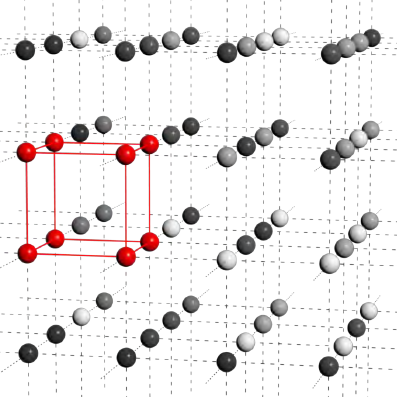
\includegraphics[width=.50\textwidth]{Wuerfel}
	\caption{Ein Wüfel im Voxelgitter \citep{SeibtBak}.}
	\label{fig:Wuerfel}
\end{figure}
\noindent Als erster Schritt im Algorithmus werden nun die Ecken und Kanten des Würfels für die spätere Verarbeitung indiziert (s. Abbildung \ref{fig:WuerfelIndizierung}).
\begin{figure}[H]
	\centering
	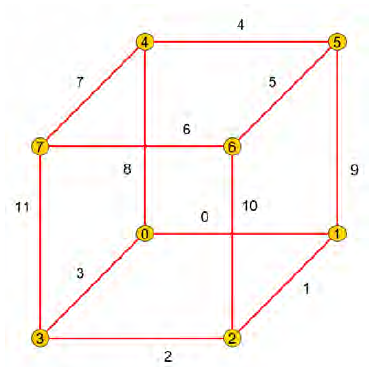
\includegraphics[width=.50\textwidth]{WuerfelIndizierung}
	\caption{Indizierung eines Würfels \citep{SeibtBak}.}
	\label{fig:WuerfelIndizierung}
\end{figure}

\noindent Jede Ecke des Würfels kann aufgrund seines Isowertes als Solide bzw. Transparent klassifiziert werden. Folglich sind aufgrund der Zwei möglichen Werte jeder Ecke $2^{8} = 256$ unterschiedliche Konfigurationen der Eingabemenge möglich. Jede dieser Konfigurationen kann als ein 8 Bit Muster dargestellt werden wobei gilt, dass jedes Bit \textit{i} bei welchem der Isowert \textit{$d_{i}$} des dazugehörigen Voxel einen gewissen Schwellwert \textit{c} überschreitet als binäre 0 interpretiert wird. Für die Werte kleiner gleich des Schwellwertes wird eine Binäre 1 angenommen.\\
\\ 
Betrachtet man nun dieses Bitmuster als natürliche Zahl erhält man einen sogenannten Würfelindex welcher einen Wert zwischen 0  und 255 aufweist dieser ist für die weitere Verarbeitung essentiell.\\
\\
Aufgrund der Symmetrie eines Würfels können durch Rotation bzw. Spiegelung die Anzahl der 255 möglichen Anordnungen der Voxeln auf 15 unterschiedliche Konfigurationen reduziert werden. Diese 15 Konfigurationen sind in Abbildung \ref{fig:MCPos} zu sehen.

\begin{figure}[H]
	\centering
	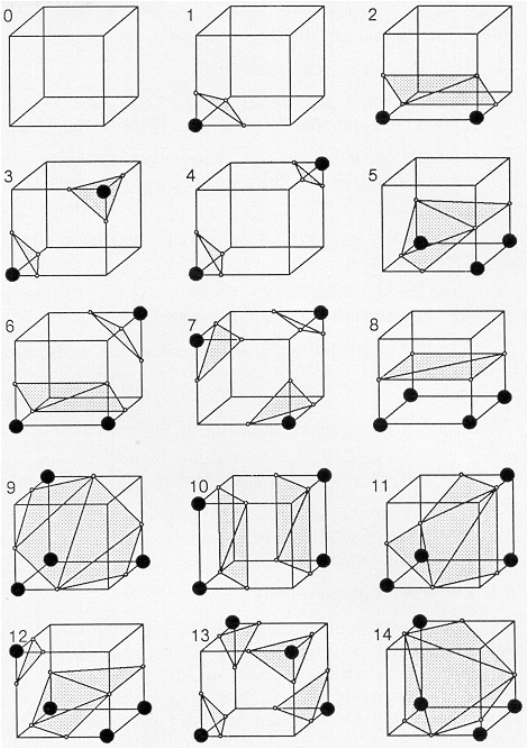
\includegraphics[width=.70\textwidth]{MCPos}
	\caption{Marching Cubes Grundkonfigurationen \citep{MCAlgo}.}
	\label{fig:MCPos}
\end{figure}

\subsubsection{Verarbeitung}
In diesem Abschnitt wird nun auf die zu durchlaufenden Schritte eines jeden Würfels aus dem Voxelgitter eingegangen. Der Ablauf lässt sich laut \citep{MCAlgo} in sieben Schritte unterteilen:\\
\begin{enumerate}
	\item Einlesen von vier Scheiben in den Speicher.
	\item Betrachten von zwei Scheiben und bilden eines Würfels aus vier Nachbarn der ersten und weiteren vier Nachbarn der zweiten Scheibe.
	\item Berechnen des Index des Würfels durch vergleichen der Isowerte der Punkte mit dem Schwellwert.
	\item Bestimmung der Liste der Dreiecksvertices anhand des Index (Abgleich mit Lookuptable).
	\item Interpolation der Positionen der Dreiecksvertices.
	\item Interpolation der Normalen an den Dreiecksvertices.
	\item Speichern der resultierenden Dreiecke und Normalen.\\
\end{enumerate}

\noindent Wie bereits im Abschnitt ''Vorbereitung'' erklärt wird in den ersten drei Punkten ein Würfel aus dem Voxelgitter extrahiert. Im Anschluss wird dieser Indexiert und jede Ecke mit einem Iso-Schwellwert abgeglichen. Der dadurch erhaltene Index wird nun in Punkt 4 für die weitere Verarbeitung benötigt. \\
\\
Punkt 4 beschreibt, dass für jede der 256 möglichen Kombinationen des Würfels die dazugehörigen Dreiecksvertices bestimmt werden müssen. Dies erfolgt durch Betrachtung zweier benachbarten Punkte des Würfels und deren Abgleich mit dem gegeben Schwellwert. Da eine erneute Auswertung für jeden Würfel äußerst rechenintensiv wäre, wird hierzu auf einen sogenannten Lookuptabel zurückgegriffen, welcher für jeden der 256 Konfigurationen die vorberechneten Werte beinhaltet. \\
\\
In Schritt 5 wird durch die Interpolation der Dreiecksverices eine Glättung der Oberfläche erreicht.\\
\\
Punkt 6 dient dazu die Position der Dreiecke im Raum zu bestimmen. Für eine nähere Beschreibung der Berechnung siehe \citep{MCAlgo}.\\
\\
Im letzten Schritt können nun die Berechneten Dreiecke weiterverwendet werden. In unserem konkreten Fall heißt das wir können das Objekt via OpenGL visualisieren und oder das Ergebnis als .stl Datei persistieren.

\subsection{Schwachpunkte}
\label{sec:schwach}
Die Grundform des Marching Cubes Algorithmus hat einige Schwachpunkte. Im laufe der Zeit wurden daher Methoden geschaffen diese Schwachstellen auszumerzen. In diesem Abschnitt werden einige Probleme aufgezählt und auf Lösungen für diese verwiesen.

\subsubsection{Uneindeutigkeit}
Die Einteilung in die 15 Grundkonfigurationen (s. Abbildung \ref{fig:MCPos}) kann zu Uneindeutigkeiten bezüglich der Repräsentation führen. Bei nicht Behandlung dieser kann es zu ''Löchern'' in der Oberfläche des resultierenden Objektes kommen. Zur Behebung dieses Problems stützen sich moderne Implementierungen des Marching Cubes Algorithmus wird daher auf Arbeiten wie \citep{Leak1} oder \citep{Leak2} zurückgegriffen welche diesbezüglich Lösungen anbieten.
\subsubsection{Dreiecksdezimierung}
Der Marching Cubes Algorithmus erzeugt von Natur aus eine sehr hohe Anzahl an Dreiecken. Dies wirkt sich negativ auf die Performanz des Algorithmus aus. Daher wurden Methoden entwickelt die es ermöglichen die Anzahl der zu verarbeitenden Dreiecke zu minimieren. Ein mögliches Verfahren zur Dezimierung ist das in \citep{DecTri} beschriebene.
\subsubsection{Glättung Dreiecksnetz}
Der Punkt der Verarbeitung ''Interpolation der Positionen der Dreiecksvertices'' welcher im Kapitel zuvor erwähnt wurde, dient bereits der Glättung des Dreiecksnetzes, da der Marching Cubes Algorithmus ohne diesen Schritt eine sehr kantige Oberfläche erzeugen würde. Um eine weitere Verfeinerung zu erreichen bietet sich hier der häufig verwendete Humphrey’s Classes Algorithmus \citep{Verf} an.
\subsubsection{Alternative Datenstruktur}
Da ein Volumen Datensatz verhältnismäßig große Ausmaße annehmen kann, bietet sich ein sogenannter Octree für eine vereinfachte Datenhaltung an. In \citep{Octree} ist die Verwendung einer solchen Struktur zur Generierung von Isoflächen dargestellt.

\section{Dateiformate}
\label{sec:DateiEinf}
Die zu dieser Arbeit herangezogenen Dateiformate sind einerseits die von dem Softwarepaket Analyze\footnote{https://rportal.mayo.edu/bir/} verwendeten Image und Header Files sowie die sogenannte STereoLithography-Schnittstelle. 

\subsection{Image File (.img)}
Diese Datei ist vergleichsweise einfach aufgebaut und enthält ein Objekt bestehend aus (normalerweise) unkomprimierten Pixel Daten (vgl. \citep{AnalyzeFormat}). Jedes Pixel repräsentiert eine Voxel mit dem jeweils dazugehörigen Isowert. Das gesamte Objekt kann somit in eine 3x3 Matrix eingelesen und verarbeitet werde.

\subsection{Header File (.hdr)}
\label{sec:DateiHead}
Diese Datei beschreibt die Ausmaße der Pixel-Datei (.img) sowie ihre Historie. (vgl. \citep{AnalyzeFormat}). \\\\
Die genaue Struktur nach \citep{AnalyzeFormat} ist in drei Teilbereiche aufgeteilt. Der erste Teil ist der sogenannte ''header key'' und beinhaltet allgemeine Informationen bezüglich der Datei (s. \ref{prog:headerKey}). Der zweite Teil beinhaltet Informationen bezüglich der Dimension der Image-Datei(s. \ref{prog:imageDim}. Der dritte und letzte Abschnitt hält Informationen bezüglich der Historie (s. \ref{prog:dataHist}).

\begin{program}[H]
	\caption{Header key als C-Struktur \citep{AnalyzeFormat}}
	\label{prog:headerKey}
	\begin{CCode}
struct header_key /* header key */
{ /* off + size */
	int sizeof_hdr /* 0 + 4 */
	char data_type[10]; /* 4 + 10 */
	char db_name[18]; /* 14 + 18 */
	int extents; /* 32 + 4 */
	short int session_error; /* 36 + 2 */
	char regular; /* 38 + 1 */
	char hkey_un0; /* 39 + 1 */
}; /* total=40 bytes */ 
	\end{CCode}
\end{program}

\begin{program}
	\caption{Data history als C-Struktur \citep{AnalyzeFormat}}
	\label{prog:dataHist}
	\begin{CCode}
struct data_history
{ /* off + size */
	char descrip[80]; /* 0 + 80 */
	char aux_file[24]; /* 80 + 24 */
	char orient; /* 104 + 1 */
	char originator[10]; /* 105 + 10 */
	char generated[10]; /* 115 + 10 */
	char scannum[10]; /* 125 + 10 */
	char patient_id[10]; /* 135 + 10 */
	char exp_date[10]; /* 145 + 10 */
	char exp_time[10]; /* 155 + 10 */
	char hist_un0[3]; /* 165 + 3 */
	int views /* 168 + 4 */
	int vols_added; /* 172 + 4 */
	int start_field; /* 176 + 4 */
	int field_skip; /* 180 + 4 */
	int omax, omin; /* 184 + 8 */
	int smax, smin; /* 192 + 8 */
}; 
	\end{CCode}
\end{program}

\begin{program}[H]
	\caption{Image Dimension als C-Struktur \citep{AnalyzeFormat}}
	\label{prog:imageDim}
	\begin{CCode}
struct image_dimension
{ /* off + size */
	short int dim[8]; /* 0 + 16 */
	short int unused8; /* 16 + 2 */
	short int unused9; /* 18 + 2 */
	short int unused10; /* 20 + 2 */
	short int unused11; /* 22 + 2 */
	short int unused12; /* 24 + 2 */
	short int unused13; /* 26 + 2 */
	short int unused14; /* 28 + 2 */
	short int datatype; /* 30 + 2 */
	short int bitpix; /* 32 + 2 */
	short int dim_un0; /* 34 + 2 */
	float pixdim[8]; /* 36 + 32 */
	/*
	pixdim[] specifies the voxel dimensitons:
	pixdim[1] - voxel width
	pixdim[2] - voxel height
	pixdim[3] - interslice distance
	...etc
	*/
	float vox_offset; /* 68 + 4 */
	float funused1; /* 72 + 4 */
	float funused2; /* 76 + 4 */
	float funused3; /* 80 + 4 */
	float cal_max; /* 84 + 4 */
	float cal_min; /* 88 + 4 */
	float compressed; /* 92 + 4 */
	float verified; /* 96 + 4 */
	int glmax,glmin; /* 100 + 8 */
}; /* total=108 bytes */ 
	\end{CCode}
\end{program}

\subsection{STereoLithography (.stl)}
\begin{quote}
	''The STL (STereoLithography) file format, as developed by 3D Systems, has been widely used by most Rapid Prototyping (RP) systems and is supported by all major computer-aided design (CAD) systems.'' - \citep{STereoLithography}
\end{quote}
Eine STL-Datei besteht im Prinzip aus einer liste von Dreiecken. Jedes Dreieck wird durch seine drei Eckpunkte im Raum (jeweils x, y und z Position) sowie durch seinen Normalvektor beschrieben. Dies führt folglich zu einer Summe von 12 Werten pro Dreieck.\\
\\
Zum besseren Verständnis kann in Abbildung \ref{fig:ASCIISTL} der Aufbau einer solchen Datei als ASCII Darstellung betrachtet werden. 

\begin{figure}[H]
	\centering
	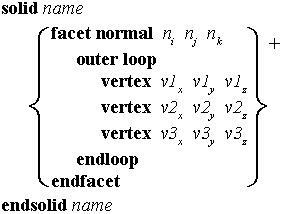
\includegraphics[width=.65\textwidth]{StL-ASCII}
	\caption{ASCII Darstellung des STL-Format \citep{STLFormat}.}
	\label{fig:ASCIISTL}
\end{figure}
\noindent Für ein besseres Verständnis hinsichtlich der Implementierung ist in Abbildung \ref{fig:BINARYSTL} der Binäre Aufbau des STL-Formates dargestellt. 
\begin{figure}
	\centering
	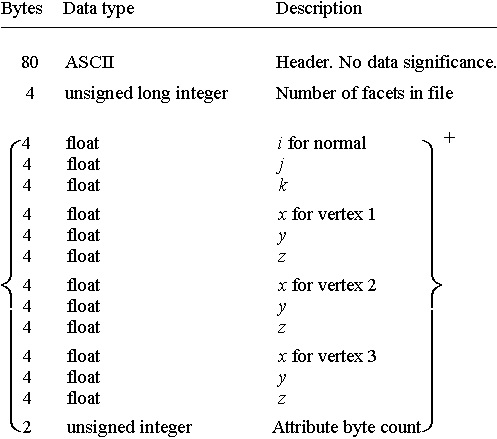
\includegraphics[width=.65\textwidth]{StL-binary}
	\caption{Binäre Darstellung des STL-Format \citep{STLFormat}.}
	\label{fig:BINARYSTL}
\end{figure}

\section{Computergrafik}
Computergrafik beschreibt das computergestützte Erstellen und Verarbeiten von Grafiken (vgl. \citep{ComputerGraphics}). In dieser Arbeit wird auf die Verarbeitung und insbesondere auf die Darstellung von dreidimensionalen Objekten als Polygon-Menge zurückgegriffen. Zu diesem Zweck bieten sich diverse Programmierschnittstellen wie OpenGL\footnote{https://www.opengl.org/}, Direct3D\footnote{https://msdn.microsoft.com/en-us/library/windows/desktop/bb153256(v=vs.85).aspx} oder AMD Mantle\footnote{http://www.amd.com/de-de/innovations/software-technologies/technologies-gaming/mantle} an, welche für Grafikausgaben genutzt werden können. Aufgrund der Aufgabenstellung dieser Arbeit findet OpenGL Verwendung.
\subsection{OpenGL}
\begin{quote}
	''OpenGL (for “Open Graphics Library”) is a software interface to graphics hardware.
	The interface consists of a set of several hundred procedures and functions
	that allow a programmer to specify the objects and operations involved in producing
	high-quality graphical images, specifically color images of three-dimensional
	objects.'' - \citep{OpenGLDoku}
\end{quote}
OpenGL ermöglicht eine verhältnismäßig einfache Plattform unabhängige Grafikprogrammierung. Da es sich um eine reine Grafikbibliothek handelt kümmert sich OpenGL nicht um die Verwaltung von Zeichenoberflächen, Renderkontexten oder weitere Puffer. Um OpenGL im Weiteren vernünftig mit einem Betriebssystem zu verwenden existieren daher verschiedene Bibliotheken. Die in dieser Arbeit verwendete Bibliothek ist QT. Die Gründe für diese Entscheidung sind die Unabhängigkeit bezüglich Betriebssystem, die Aktualität der Bibliothek sowie die hohe Verbreitung dieser.